\chapter{Introduction}

Smartphones nowadays are capable of doing a multitude of tasks which was not possible with conventional phones, With the increase in complexity of smartphones, We can now send emails, click high-definition photos, Access satellite navigation and remain connected to the outside world 24 x 7.  The capabilities which makes smartphones different from conventional phones is giving nightmares to security organisations in tracing and extracting data from the smartphones.  The criminals are now  able to wipe out the traces of criminal activities performed using their phones with much ease than before.  The criminal organisations are also using smartphones to communicate with others using encrypted messages which are very hard to trace and decrypt.  Even if the phones are confiscated after the crime, It is becoming very hard for law-enforcement agencies to extract data from those devices as these devices are encrypted with advanced encryption features and any attempt to get access to the device memory using brute-force would potentially wipe the all the data inside and overwrite it with 0. In this scenario, A radically new approach is necessary to proactively monitor the criminal activities with minimal interference and maximum stealth.

\section{Smartphone OS Market Share}

According to Gartner ,it's estimated that there are roughly 2 billion smartphone users in the market (1.91 billion to be exact), with that number expected to increase another 12\% in 2016 to top 2.16 billion people globally. The global share of smartphone OS is as follows:

\begin{figure}
   \vspace*{-1cm}
    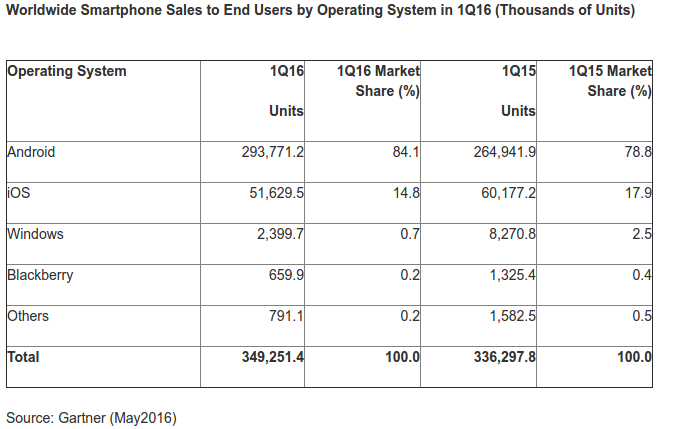
\includegraphics[height=0.5\textheight]{Figures/fig01/gartner}
    \caption{\href{http://www.gartner.com/newsroom/id/3323017} Gartner Survey Results}
    \label{gartner}
   
    
  \end{figure}


Android dominated the smartphone market with a share of 84 \% , IOS with 14.8 \% and Windows with 0.7\% of the Global smartphone market.As we can see Android OS is the most popular smartphone OS with almost 84 \% market share and hence we  are interested in examining the forensics capabilities in Android OS. 
\goodbreak
\section{Android Architecture}
Android is a mobile operating system developed by google based on the linux kernel and designed primarily for touchscreen mobile devices. Android source code is open-source and it is one of the main reason of the immense popularity of the android OS.
\begin{figure}
   \vspace*{-1cm}
    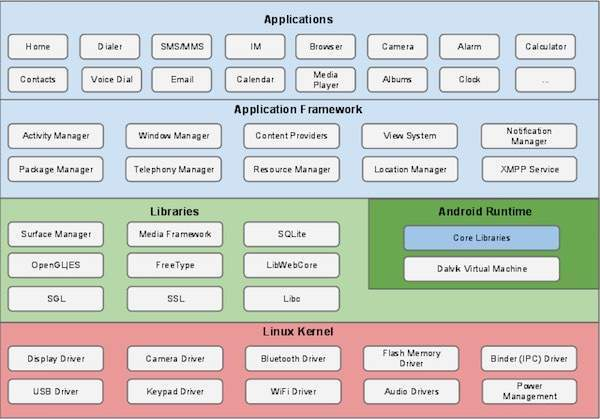
\includegraphics[height=0.5\textheight]{Figures/fig01/architecture}
    \caption{\href{https://www.tutorialspoint.com/android/}{Android Architecture} }
    
   
    
  \end{figure}


\subsection{Linux Kernel}
The basic layer is the Linux kernel. The whole Android OS is built on top of the Linux 3.x Kernel with some further architectural changes made by Google. It is this Linux that interacts with the hardware and contains all the essential hardware drivers. Drivers are programs that control and communicate with the hardware. For example, consider the Bluetooth function. All devices has a Bluetooth hardware in it. Therefore the kernel must include a Bluetooth driver to communicate with the Bluetooth hardware. The Linux kernel also acts as an abstraction layer between the hardware and other software layers. Android uses the Linux for all its core functionality such as Memory management, process management, networking, security settings etc. As the Android is built on a most popular and proven foundation, it made the porting of Android to variety of hardware, a relatively painless task.


\subsection{Libraries}
The next layer is the Android native libraries. It is this layer that enables the device to handle different types of data. These libraries are written in c or c++ language and are specific for a particular hardware.Some of the important native libraries include the following: 
\begin{itemize}

  \item \textbf{Surface Manager:} It is used for compositing window manager with off-screen buffering means you can't directly draw into the screen, but your drawings go to the off-screen buffer. There it is combined with other drawings and form the final screen the user will see. This off screen buffer is the reason behind the transparency of windows.

  \item \textbf{Media framework:} Media framework provides different media codecs allowing the recording and playback of different media formats.

  \item \textbf {SQLite:} SQLite is the database engine used in android for data storage purposes.

  \item \textbf{WebKit:} It is the browser engine used to display HTML content.

  \item\textbf{ OpenGL:} Used to render 2D or 3D graphics content to the screen.

  

\end{itemize}



\subsection{Android Runtime}

Android Runtime consists of Dalvik Virtual machine and Core Java libraries. 

\begin{itemize}

	\item \textbf{Dalvik Virtual Machine:}  It is a type of JVM used in android devices to run apps and is optimized for low processing power and low memory environments. Unlike the JVM, the Dalvik Virtual Machine does not run .class files, instead it runs .dex files. .dex files are built from .class file at the time of compilation and provides higher efficiency in low resource environments. The Dalvik VM allows multiple instance of Virtual machine to be created simultaneously providing security, isolation, memory management and threading support. It is developed by Dan Bornstein of Google. 

	Android 4.4 introduced Android Runtime (ART) as a new runtime environment, which uses ahead of time (AOT) compilation to entirely compile the application bytecode into machine code upon the installation of an application.

	

	\item \textbf{Core Java Libraries:} These are different from Java SE and Java ME libraries. However these libraries provides most of the functionalities defined in the Java SE libraries.

\end{itemize}

\subsection{Application Framework}

These are the blocks that our applications directly interacts with. These programs manage the basic functions of phone like resource management, voice call management etc.  Important blocks of Application framework are:

\begin{itemize}

\item \textbf{Activity Manager:}Manages the activity life cycle of applications.

\item \textbf{Content Providers:} Manage the data sharing between applications.

\item \textbf{Location Manager:} Location management, using GPS or cell tower .

\item \textbf{Resource Manager:} Manage the various types of resources we use in our Application.



\end{itemize}





\subsection{Applications}

Applications are the top layer in the Android architecture and this is where our applications are going to fit. Several standard applications comes pre-installed with every device, such as: 

\begin{itemize}

\item SMS client 

\item App Dialer

\item Web browser

\item Contact manager
\end{itemize}

\subsection{Applications Used in Criminal Activites}
The Criminals are increasingly becoming tech savvy and are using various apps which provide encryption facilities and as well as secure communication.This is becoming a problem for security agencies as they are not able to intercept the communication channel. .Some of the apps used by Criminals Networks are as follows:

\begin{itemize}
\item \textbf{Mappr} An App that can change location data on photos, so they don't reveal where they actually are.
\item \textbf{Cryptophone }An App that uses end-to-end encryption to for phone calls which effectively means that except the two communicating parties , no other person will be able the decrypt the data stream.
\item \textbf{Telegram} An  encrypted mobile messaging app that can host different channels where  members can talk in a group setting.
\item \textbf{Firechat} An App that connects to nearby devices which have firechat installed through wifi or bluetooth and build a "mesh network" that allows messages to be passed to other devices within vicinity without any usage of cell phone tower.
\end{itemize}


\clearpage

% -eof-
